\documentclass[tikz,border=10pt]{standalone}

\usepackage{fontspec}
\setmainfont{Fira Sans}[
    BoldFont   = {Fira Sans Bold},
    ItalicFont = {Fira Sans Italic},
    BoldItalicFont = {Fira Sans Bold Italic},
]
\setsansfont{Fira Sans}
\setmonofont{FiraCode NF}[Scale=0.85]
\renewcommand{\familydefault}{\sfdefault}

\usepackage[dvipsnames]{xcolor}
\definecolor{accent}{HTML}{3F51B5}
\definecolor{accentlight}{HTML}{C5CAE9}
\definecolor{accentdark}{HTML}{283593}
\definecolor{warnred}{HTML}{C62828}
\definecolor{exgreen}{HTML}{2E7D32}

\usepackage{hyperref}
\hypersetup{colorlinks=true, urlcolor=accent}

\usetikzlibrary{shapes.geometric, arrows.meta, positioning, calc}

\begin{document}
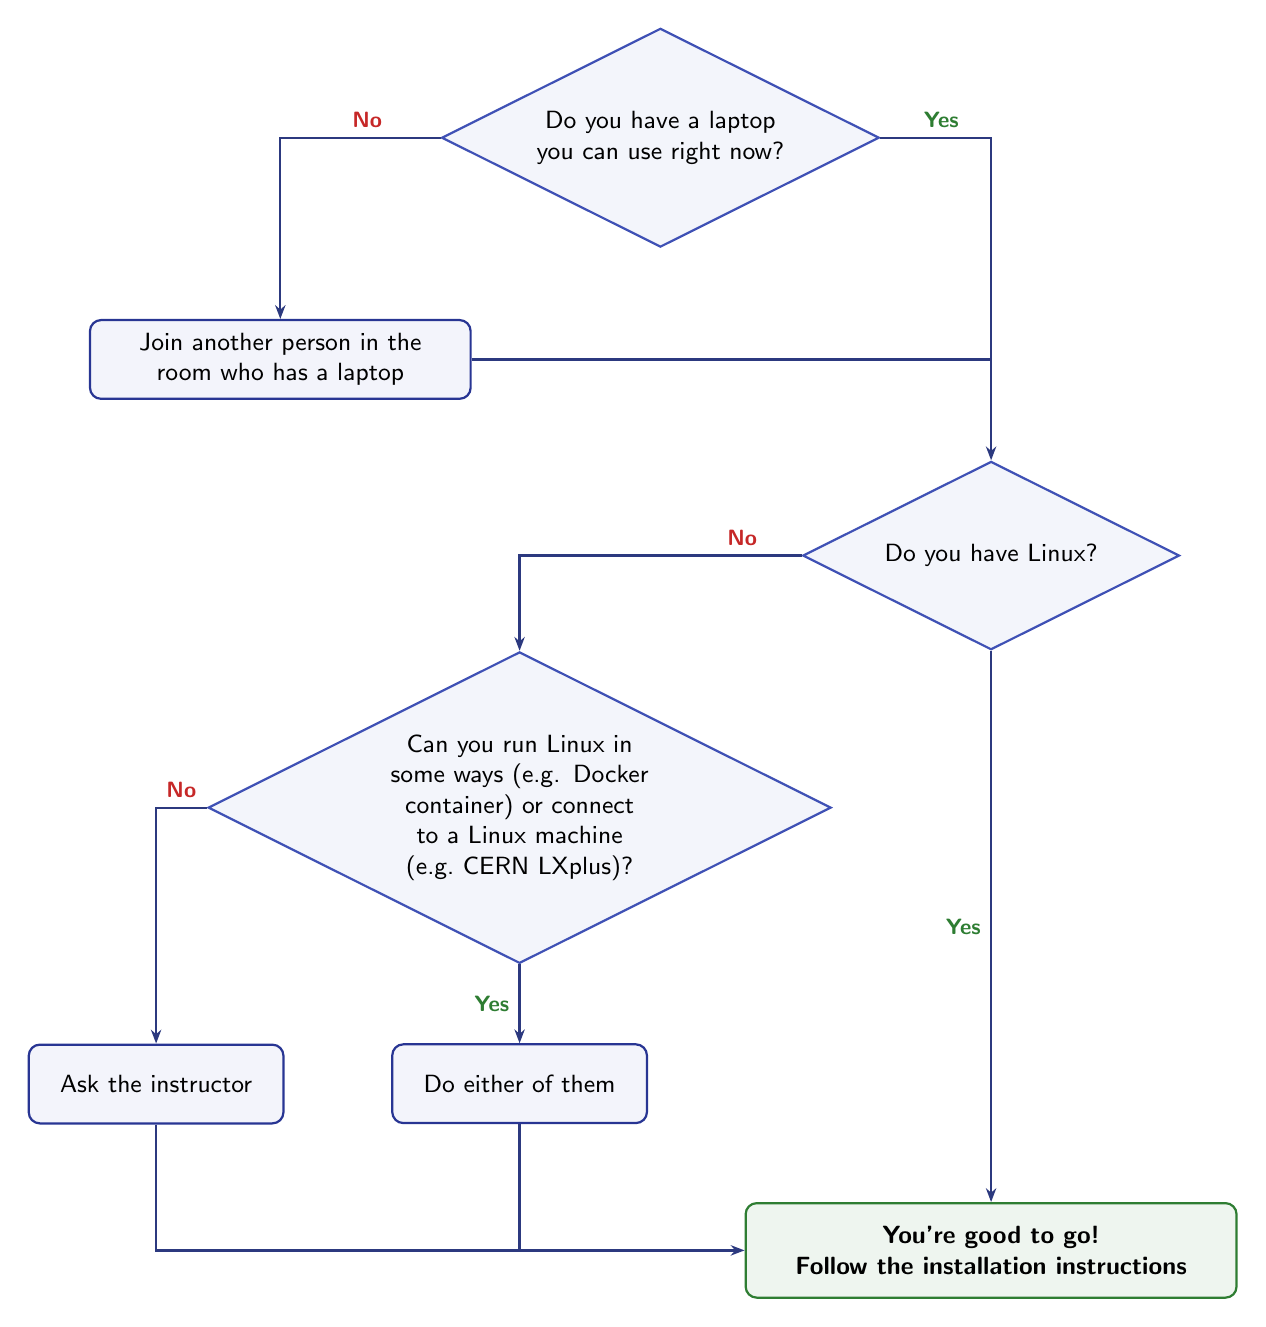
\begin{tikzpicture}[
    node distance=1.4cm and 2.8cm,
    question/.style={
        diamond,
        draw=accent,
        fill=accent!6,
        thick,
        text width=3.8cm,
        align=center,
        inner sep=2pt,
        font=\small,
        aspect=2,
    },
    action/.style={
        rectangle,
        rounded corners=4pt,
        draw=accentdark,
        fill=accentlight!20,
        thick,
        text width=4.6cm,
        align=center,
        minimum height=1cm,
        font=\small,
    },
    action2/.style={
        rectangle,
        rounded corners=4pt,
        draw=accentdark,
        fill=accentlight!20,
        thick,
        text width=3cm,
        align=center,
        minimum height=1cm,
        font=\small,
    },
    success/.style={
        rectangle,
        rounded corners=4pt,
        draw=exgreen,
        fill=exgreen!8,
        thick,
        text width=6cm,
        align=center,
        minimum height=1.2cm,
        font=\small\bfseries,
    },
    arr/.style={-{Stealth[length=5pt]}, thick, color=accent!70!black},
    lin/.style={thick, color=accent!70!black},
    yeslbl/.style={font=\footnotesize\bfseries, color=exgreen},
    nolbl/.style={font=\footnotesize\bfseries, color=warnred},
]

\node[question] (q1) {Do you have a laptop you can use right now?};

\node[action, below left=1.6cm and 1 cm of q1] (a2)
    {Join another person in the room who has a laptop};

\node[question, below right=4 cm and 1.6 cm of q1] (q3)
    {Do you have Linux?};

\node[question, below left=1.6cm and 2.8 cm of q3] (q4)
    {Can you run Linux in some ways (e.g. Docker container) or connect to a Linux machine (e.g.\ CERN LXplus)?};

\node[action2, below=1cm of q4] (a5)
    {Do either of them};

\node[action2, below left=2 cm and 1 cm of q4] (a6)
    {Ask the instructor};

\node[success, below=7cm of q3] (q7)
    {You're good to go!\\Follow the installation instructions};

\draw[arr] (q1.east) -| node[above right, yeslbl, pos=0.15] {Yes} (q3.north);
\draw[arr] (q1.west) -| node[above left, nolbl, pos=0.15] {No} (a2.north);

\coordinate (A) at ($(q3.north)+(0,5cm)$);
\draw[lin] (a2.east) -- ($(A)!(a2.east)!(q3.north)$);

\draw[arr] (q3.south) -- node[left, yeslbl] {Yes} (q7.north);
\draw[arr] (q3.west) -| node[above right, nolbl, pos=0.15] {No} (q4.north);

\draw[arr] (q4.south) -- node[left, yeslbl] {Yes} (a5.north);
\draw[arr] (q4.west) -| node[above right, nolbl, pos=0.5] {No} (a6.north);

\draw[arr] (a6.south) |- (q7.west);

\coordinate (B) at ($(q7.west)-(5cm,0)$);
\draw[lin] (a5.south) -- ($(B)!(a5.south)!(q7.west)$);

\end{tikzpicture}
\end{document}
